\documentclass{article}

\usepackage{fancyhdr}
\usepackage{hyperref}
\usepackage{titlesec}
\usepackage{graphicx}

\setcounter{secnumdepth}{4}


\pagestyle{fancy}
\fancyhf{}
\rhead{Path-finding Algorithms and Solving Mazes}
\lhead{Oliver Temple [CN]}
\rfoot{\thepage}
\lfoot{Path-finding Algorithms and Solving Mazes}

\title{Path-finding Algorithms and Solving Mazes}

\author{Oliver Temple}

\begin{document}

\maketitle
\tableofcontents

\section{analysis}
\subsection{Project Description}
Path finding algorithms are essential in many aspects computer science, especially in games and simulations. However, they can be complex things that are hard to visualize, especially when being taught about them. Path finding algorithm visualizers do exist, however, I feel that none of them are perfect, and that they lack features.

Because of this, I am going to make a path finding visualizer that ticks all of the boxes. 



\subsection{Project Background}
\subsubsection{Example 1}
\href{https://clementmihailescu.github.io/Pathfinding-Visualizer/
}{https://clementmihailescu.github.io/Pathfinding-Visualizer
}
\newline
In this example, mazes can be generated with various algorithms, as well as being drawn by the user. The mazes can also be edited after they have been generated. The available maze generation algorithms are:
\begin{itemize}
    \item Recursive Division
    \item Recursive Division (vertical skew)
    \item Recursive Division (horizontal skew)
    \item Basic Random Maze
    \item Basic Weight Maze
    \item Simple Stair Pattern
\end{itemize}
These mazes can then be solved with a number of different path finding algorithms. The available path finding algorithms are:
\begin{itemize}
    \item Djikstra's Algorithm
    \item A* Search
    \item Greedy Best-first Search
    \item Swarm Algorithm
    \item Convergent Swarm Algorithm
    \item Bidirectional Swarm Algorithm
    \item Breadth-first Search
    \item Depth-first Search
\end{itemize}
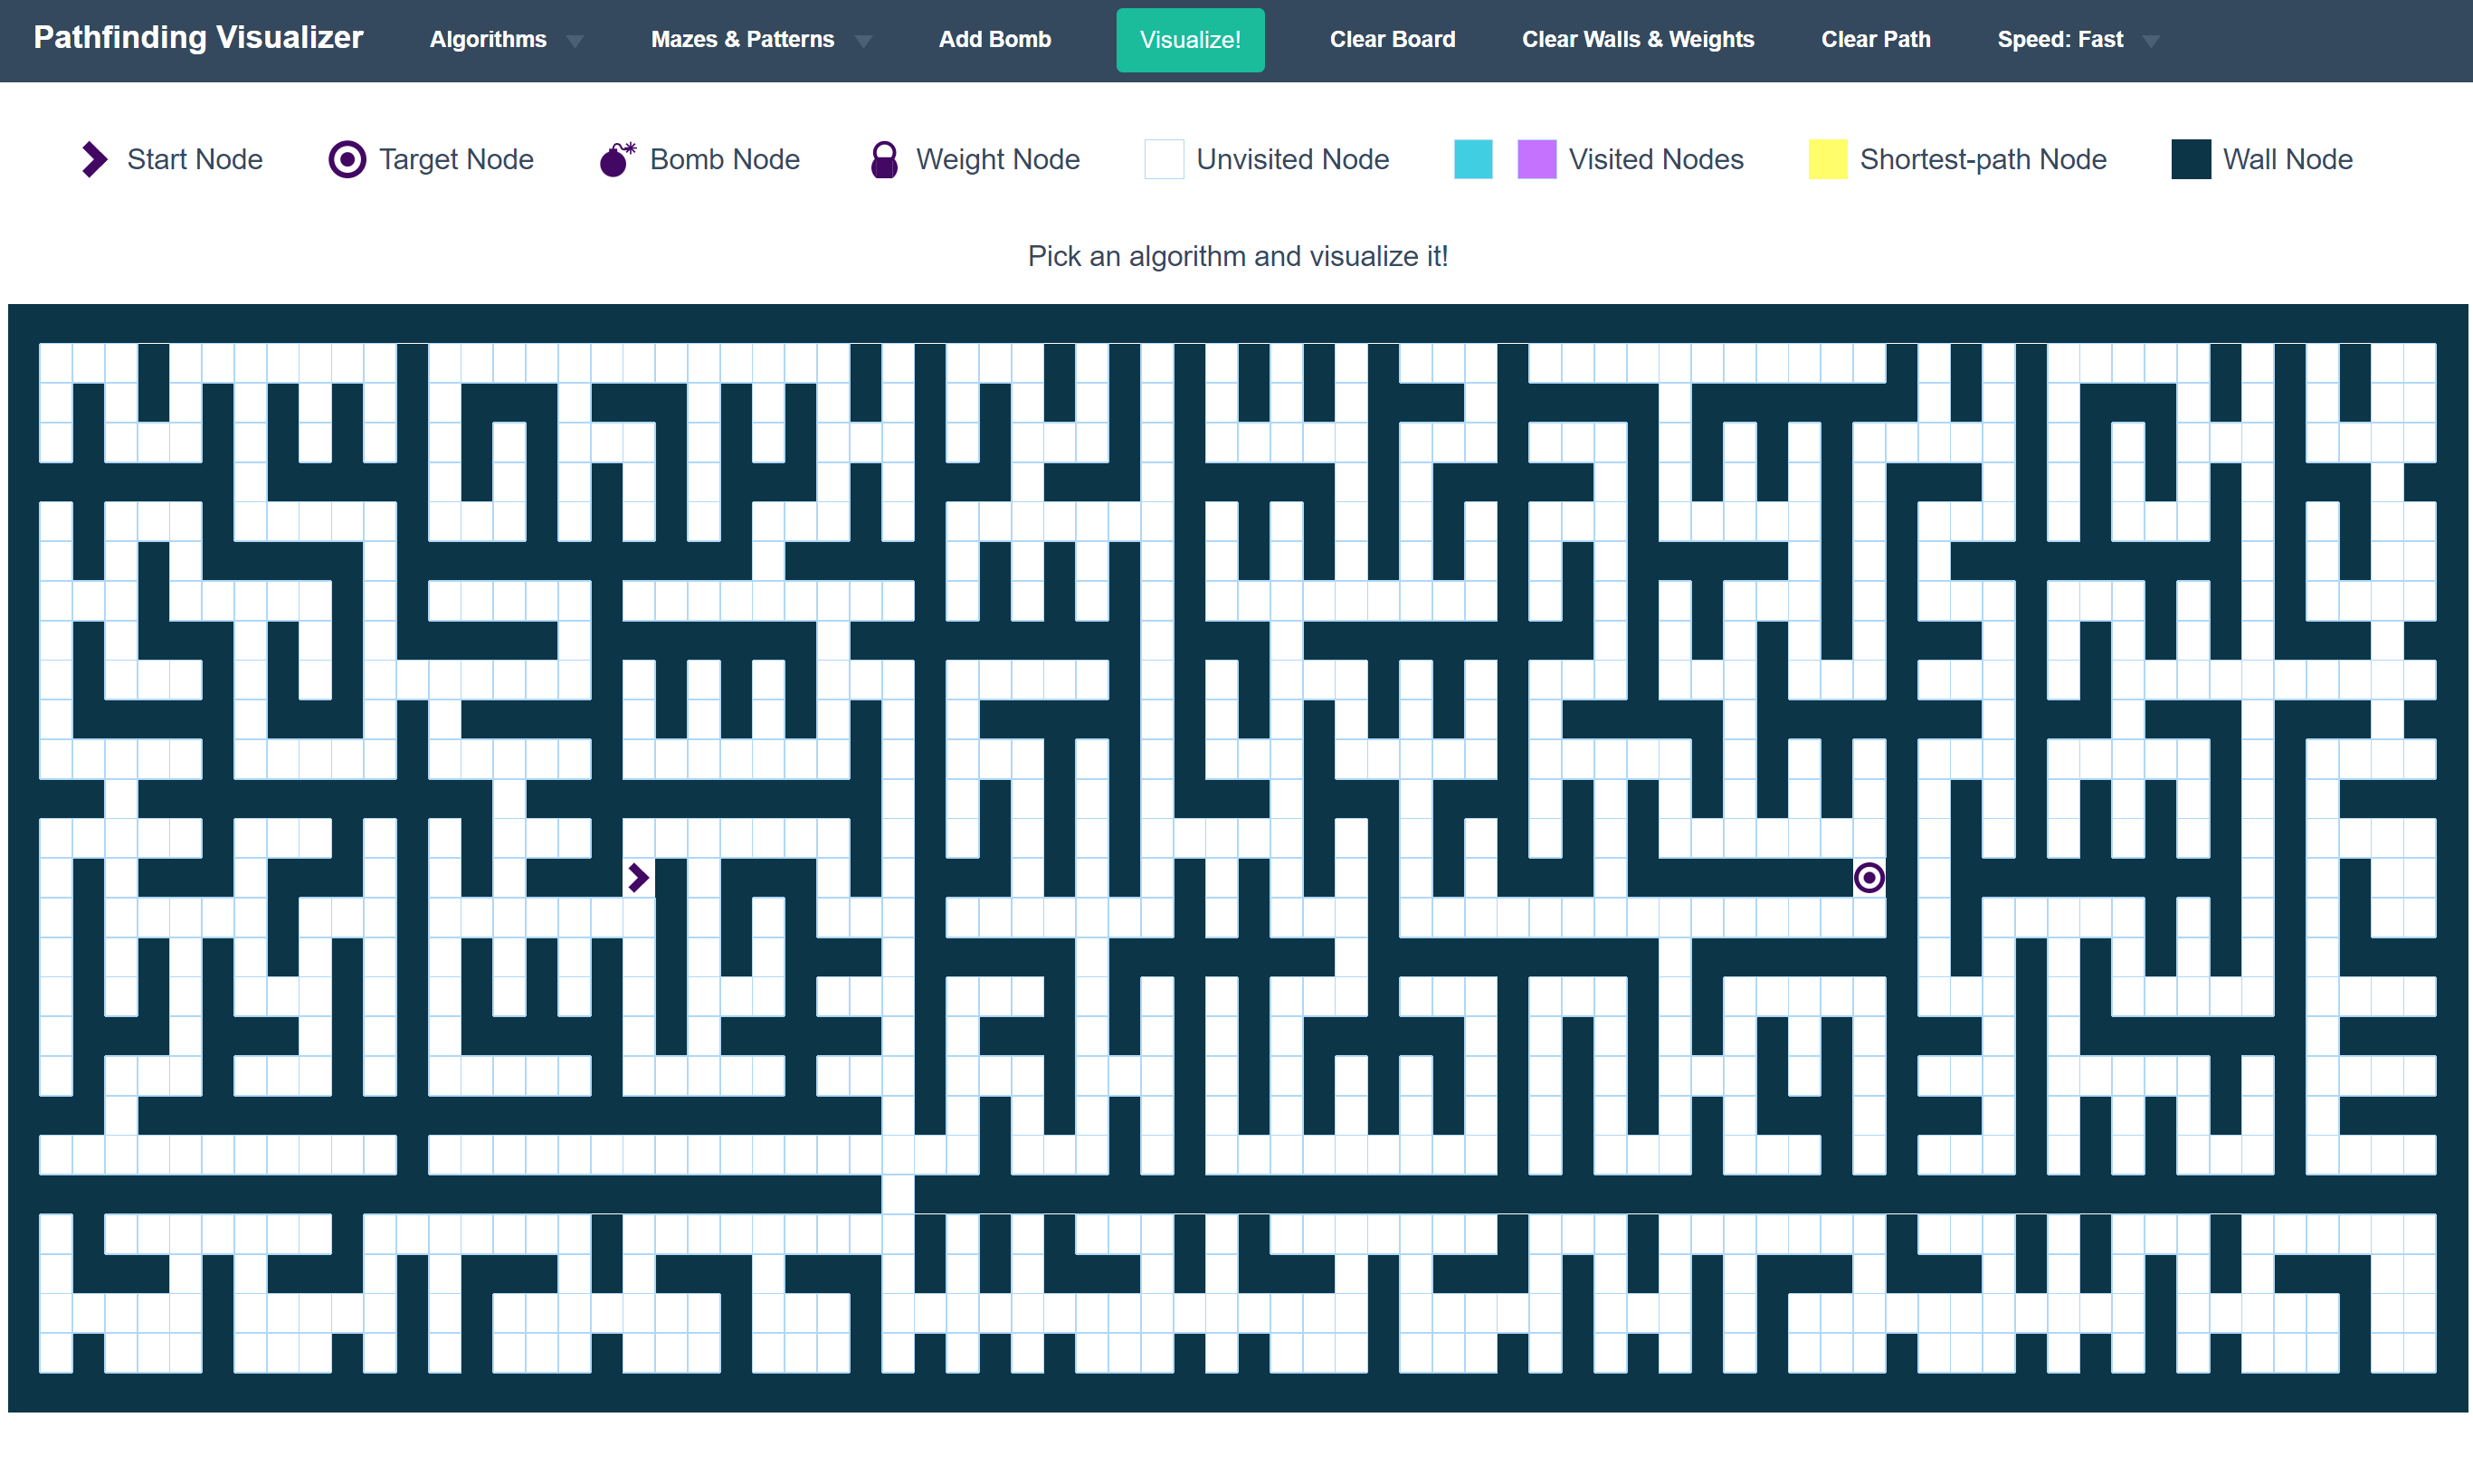
\includegraphics[width=\linewidth]{assets/Existing Solutions/example 1.PNG}
\paragraph{pros}
\begin{itemize}
    \item Many different algorithms to choose from.
    \item Start and end nodes can be moved.
    \item Maze can be altered.
    \item If nodes are moved after visualization has run, then the visualization will update.
    \item "Bomb" node, adds a via point that the path must go through.
\end{itemize}
\paragraph{cons}
\begin{itemize}
    \item The visualization is too slow.
    \item If maze is altered by user after visualization has run, then the visualization will not update.
    \item 
\end{itemize}


\subsubsection{Example 2}
\href{https://qiao.github.io/PathFinding.js/visual/
}{https://qiao.github.io/PathFinding.js/visual/
}
\newline
In this example, mazes have to be drawn by the user. The maze can then be solved with a number of different algorithms, however, these algorithms have more choice. For example, in the A* option, you can change the heuristic that is used. The available algorithms are:
\begin{itemize}
    \item A*
    \item IDA*
    \item Breadth-First-Search
    \item Best-First-Search
    \item Dijkstra
    \item Jump Point Search
    \item Orthogonal Jump Point Search
    \item Trace
\end{itemize}
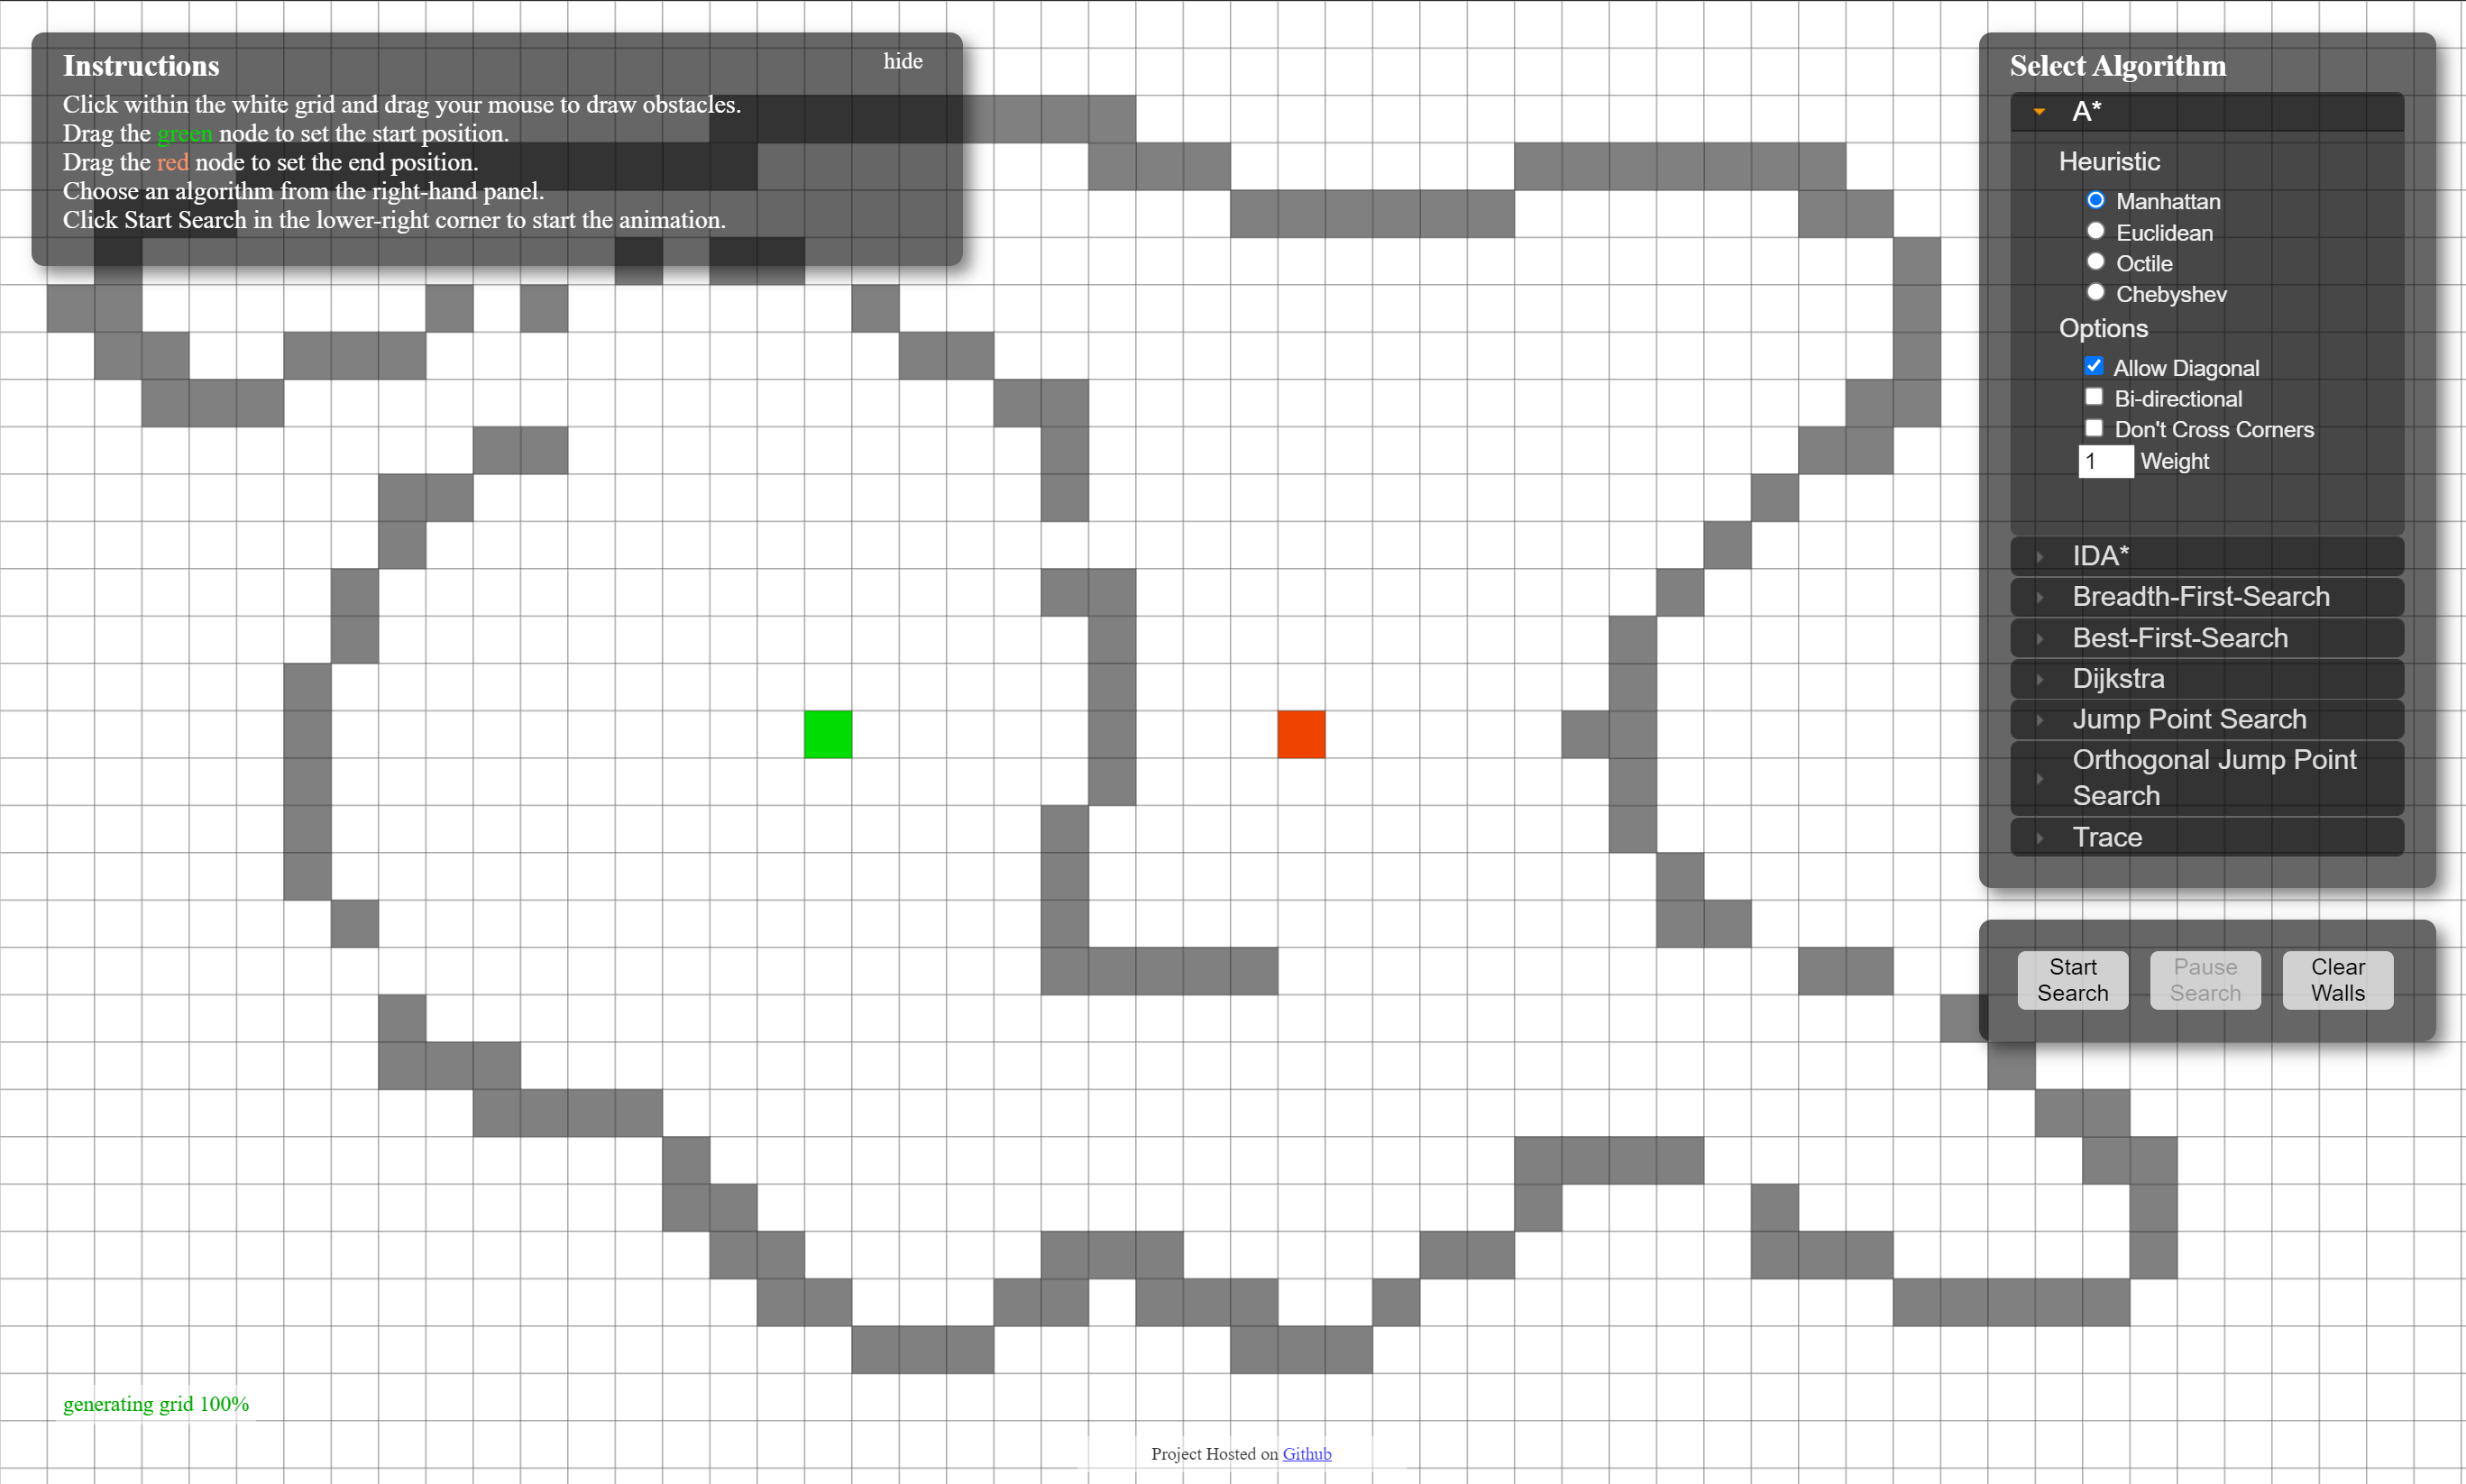
\includegraphics[width=\linewidth]{assets/Existing Solutions/example 2.PNG}
\paragraph{pros}
\begin{itemize}
    \item More options to choose from within each algorithm.
\end{itemize}
\paragraph{cons}
\begin{itemize}
    \item No maze generation.
    \item Visualization does not update when maze or start/finnish nodes are changed.
\end{itemize}


\subsubsection{Example 3}
\href{https://pathfindout.com/
}{https://pathfindout.com/
}
\newline
In this example, mazes can be generated or drawn, however, mazes can only be generated with the recursive division algorithm. There are fewer path finding algorithms to solve the mazes than the others. The available algorithms are:
\begin{itemize}
    \item Dijkstra's Algorithm
    \item A* Search
    \item Breadth First Search
    \item Depth First Search
\end{itemize}
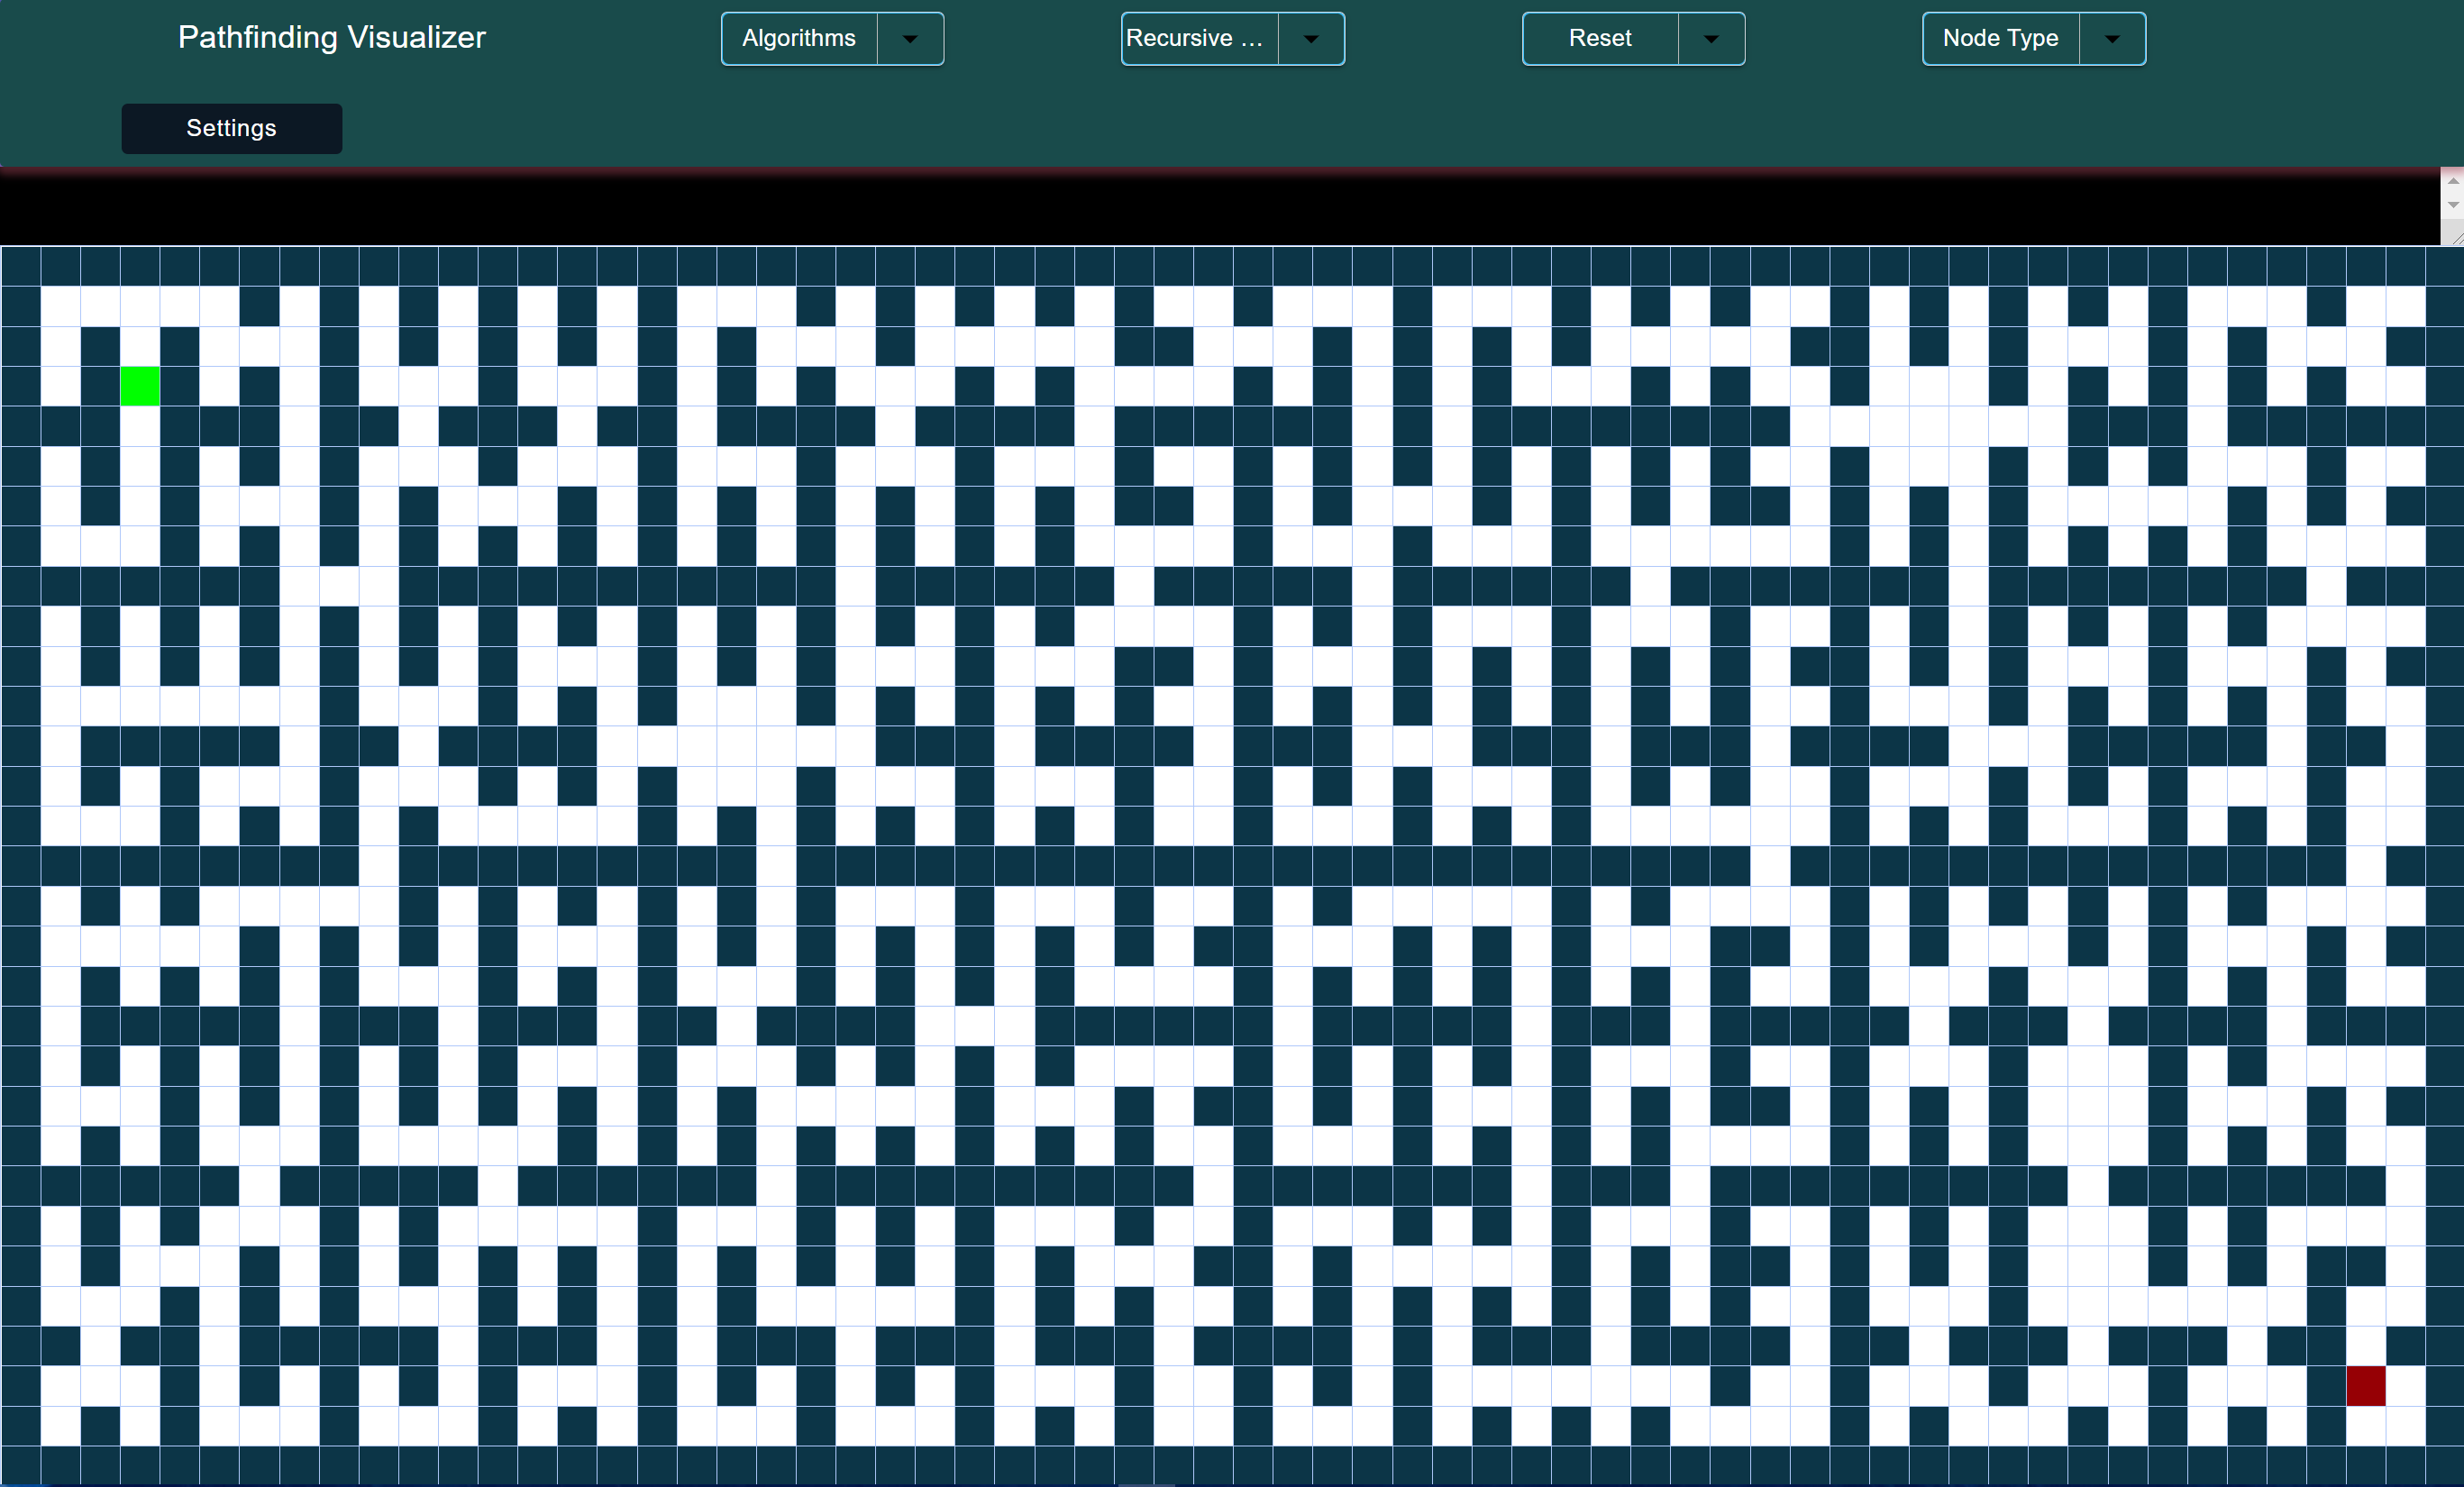
\includegraphics[width=\linewidth]{assets/Existing Solutions/example 3.PNG}
\paragraph{pros}
\begin{itemize}
    \item Different weighted nodes available.
    \item Shows how many nodes visited.
    \item Shows final path length.
    \item Data structure for some algorithms can be changed.
    \item Weights of specific node types can be changed.
    \item Node size can be changed.
\end{itemize}
\paragraph{cons}
\begin{itemize}
    \item Sometimes generates mazes that cannot be solved.
    \item Cannot edit maze after visualization has run.
    \item Only one maze generation algorithm.
    \item Fewer path finding algorithms to solve the maze.
\end{itemize}
\section{Design}

\section{Evidence of Completeness}
%out of 15 marks, argument for why the project is complete. Which algorithms have been used?
\section{Technical Solution}

\section{Testing}

\section{Evaluation}
\end{document}